\documentclass[12pt, a4paper]{article}
\title{Измерение магнитного поля Земли (3.1.3)}
\author{Стеценко Георгий, Б02-312}
\date{}
% !TeX encoding = UTF-8

\usepackage{geometry}
\usepackage{amsmath, amsfonts, amssymb, amsthm} % стандартный набор AMS-пакетов для математ. текстов
\usepackage{mathtext}
\usepackage[utf8]{inputenc} % кодировка utf8
\usepackage[russian]{babel} % русский язык
\usepackage[pdftex,dvipsnames]{xcolor} % работа с цветами
\usepackage[pdftex]{graphicx} % графика (картинки)
\usepackage{tikz,pgfplots} % рисунки
\usepackage{indentfirst}
%\usepackage[labelfont=bf,labelsep=endash,skip=3pt]{caption} % подпись картинок
% \usepackage{fancyhdr,pageslts} % настройка колонтитулов
\usepackage{enumitem} % работа со списками
\usepackage{floatrow,multicol,multirow,longtable,hhline} % работа с таблицами
\usepackage{float,wrapfig} % плавающие объекты
\usepackage{tcolorbox} % рамка вокруг текста
%\usepackage[calc]{datetime2} % дата
\usepackage{bm} % жирное начертание в формулах
\usepackage{physics} % физический пакет
\DeclareMathAlphabet\mathbfcal{OMS}{cmsy}{b}{n}
\usepackage{pgfornament} % красивые рюшечки и вензеля
\usepackage{mdframed}
\usepackage{derivative}
\usepackage{mathrsfs} %EDS
\usepackage{soul} % strikethorugh
%\usepackage{boondox-cal}

% ----------------------------------------
% Настройка шрифта

% Просто закооментируйте следующую строчку, если не работает. Будет другой шрифт, правда :(
% \usepackage{pscyr}

% ----------------------------------------
% Стилевые настройки

\usepackage{boldline} % жирная линия после таблиц (чтобы не было ошибок, этот пакет должен подключаться именно тут!)
\floatsetup[table]{style=Plaintop,floatrowsep=qquad} % настройка оформления таблиц
\setlist[enumerate,itemize]{leftmargin=5mm,itemindent=10mm,itemsep=0mm,
listparindent=0em,labelsep=2mm,topsep=2mm,labelwidth=4mm} % настройки списков

\setlength{\columnsep}{0.5cm} % расстояние между колонками
\setlength{\parskip}{1pt} % расстояние до текста от колонтитула

%\usepackage{titlesec} % управление оформлением section
%\renewcommand{\thesection}{\Roman{section}}
%\titleformat{\section}[block]{\bfseries\large}{\thesection.}{5pt}{}

% ----------------------------------------
% Настройки полей
\geometry{
  left=10mm,
  top=10mm,
  right=10mm,
  bottom=15mm,
  marginparsep=0mm,
  marginparwidth=0mm,
  headheight=0pt,
  headsep=0pt,
footskip=20pt}

% ----------------------------------------
% Настройки колонтитулов и нумерации страниц
\pagenumbering{arabic}



\newcounter{ntask}
\setcounter{ntask}{0}


\newcommand{\arsh}{\mathrm{arsh} \,\,}
\newcommand{\arch}{\mathrm{arch} \,\,}
\newcommand{\arth}{\mathrm{arth} \,\,}
\newcommand{\arcth}{\mathrm{arcth} \,\,}
\renewcommand{\Re}{\operatorname{Re} \,}
\newcommand{\EDS}{\mathscr{E}}
\newcommand{\diffract}[1]{\frac{\mathrm{d}#1}{\mathrm{d}t}}

\newcommand{\m}{\mathfrak{m}}
\newcommand{\cgs}{\quad\text{(ед. СГС)}}
\newcommand{\fcgs}{~\text{ед. СГС}}
\addto\captionsrussian{\def\refname{Источники}}

\begin{document}
	\maketitle
	
	\section{Цель работы} 
Исследование свойства постоянных неодимовых магнитов; измерение с
их помощью горизонтальную~и~вертикальную составляющие индукции магнитного поля
Земли~и~магнитное наклонение.

\section{Теоретические сведения}
Используемые в~работе постоянные магниты обладают двумя свойствами: магнитожесткостью~и~однородной намагниченностью. Это означает, что намагниченность в~любой точке шарика будет одинакова вне зависимости от~внешнего магнитного поля~и~положения точки в~шарике. Тогда известно, что вне шарика индукция магнитного поля снаружи от~шарика описывается следующей формулой:
\begin{equation}
\mathbf{B} = \frac{3(\m \cdot \mathbf{r})\cdot\mathbf{r}}{r^5} - \frac{\m}{r^3}\cgs
\label{dipole_eq}
\end{equation}

На магнитный диполь, помещённый в~магнитное поле, действует некоторая равнодействующая сила~и~магнитный момент, равные соответственно:
\begin{equation}
\mathbf{F} = (\m \cdot \nabla)\mathbf{B} 
\label{force}
\end{equation}

\begin{equation}
\mathcal{M} = \left[ \m \times \mathbf{B} \right]
\label{momentum}
\end{equation}

Из (\ref{force}) имеем выражение для~силы притяжения двух одинаковых сонаправленных магнитов, разнесённых на расстояние $h$:
\begin{equation}
\mathbf{F} = 6 \frac{\m^2}{r^4}\cgs
\label{force_eq}
\end{equation}

Кроме того, нам понадобится выражение для намагниченности (\ref{mv}) и остаточной индукцией материала магнита (\ref{br}):
\begin{equation}
	\m = \mathbf{M}V
	\label{mv}
\end{equation}
\begin{equation}
	\mathbf{B_r} = 4\pi \mathbf{M} \cgs
	\label{br}
\end{equation}

\section{Методика измерений}
\textbf{В работе используются:} неодимовые магниты; тонкая нить для~изготов­
ления крутильного маятника; медная проволока; электронные весы; секун­
домер; измеритель магнитной индукции; штангенциркуль; брусок, линейка
и штатив из немагнитных материалов; набор гирь~и~разновесов.
\newpage
\subsection{Определение магнитного момента}
\begin{wrapfigure}[8]{r}{4.5cm}\vspace{-12mm}
\centering
	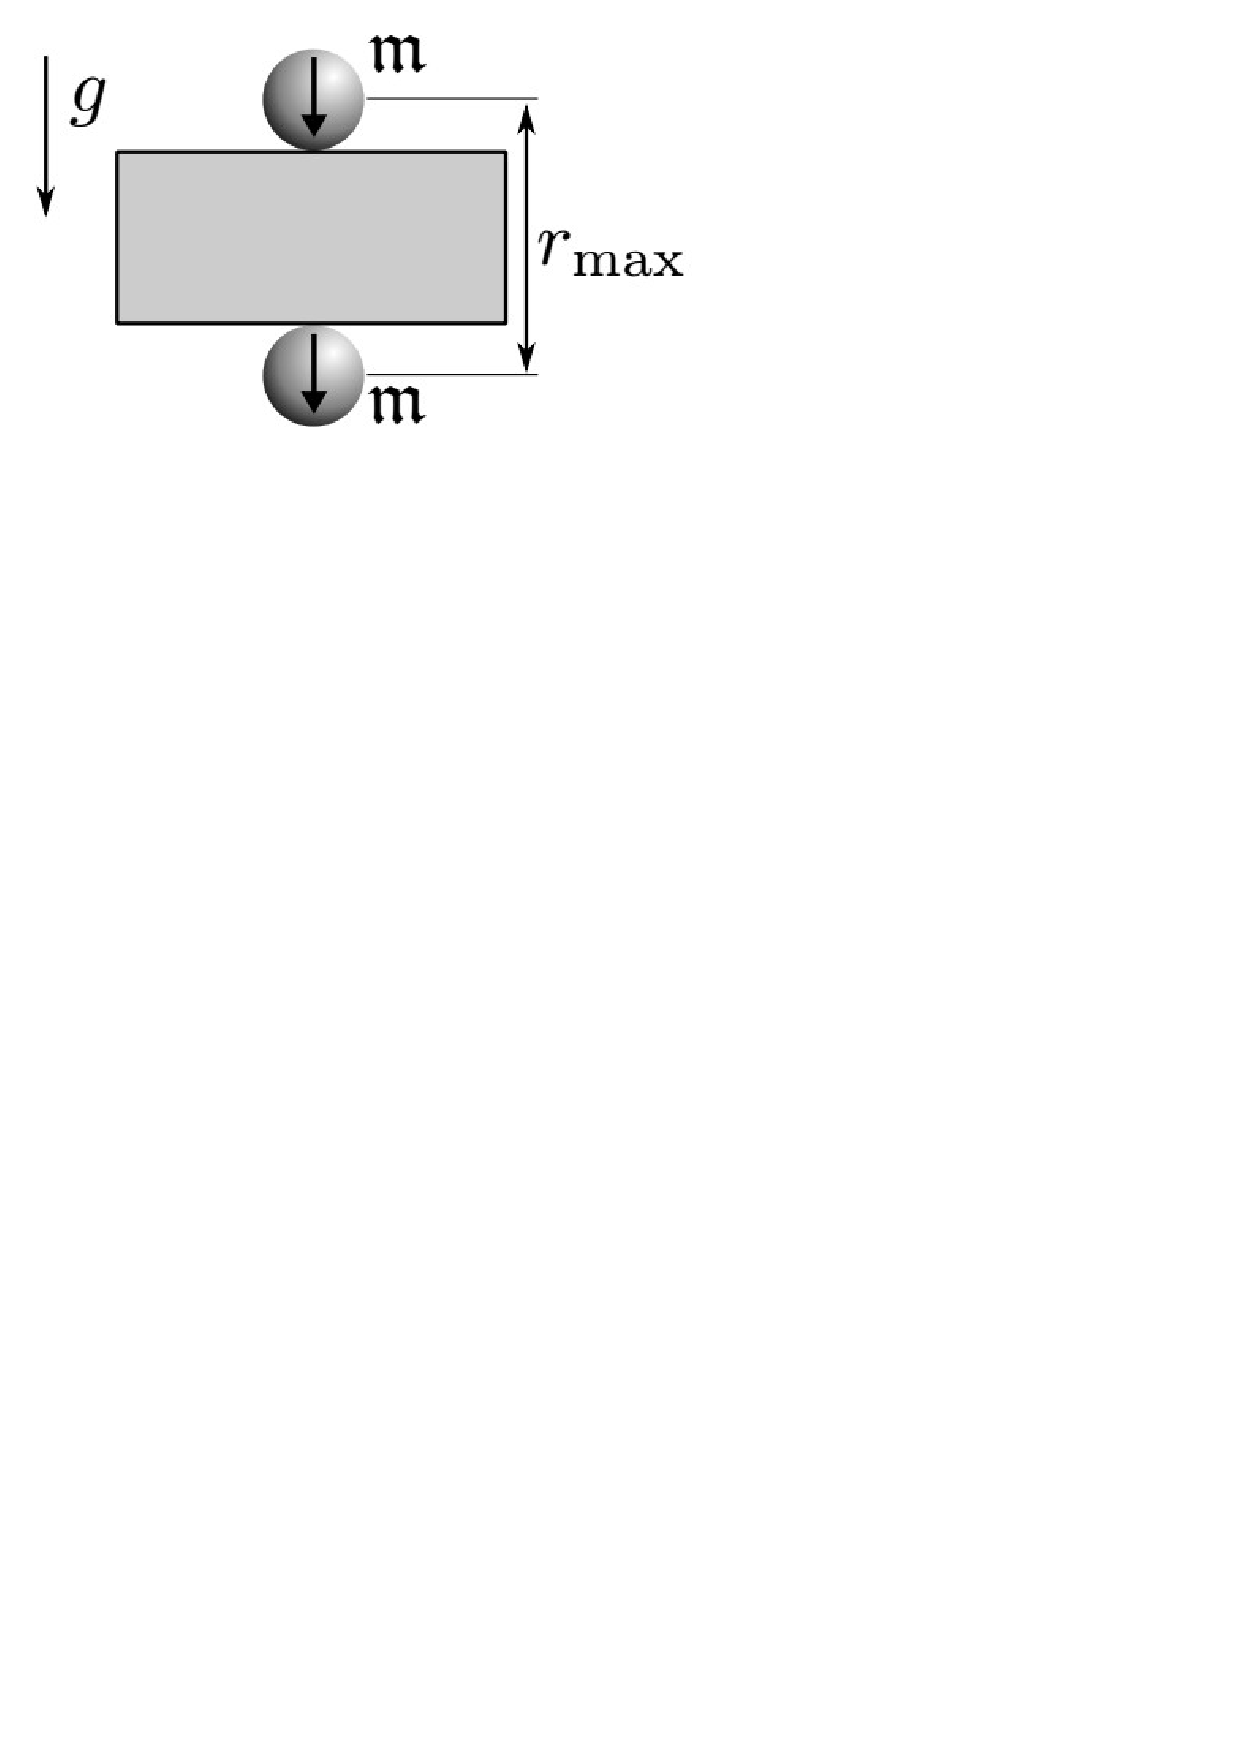
\includegraphics[width=4cm]{pics/m_offset.pdf}
	\caption{Первый способ определения магнитного момента.}
	\label{m_offset_pic}
\end{wrapfigure}

\textbf{1-й способ.} Величину магнитного момента $\m$ двух одинаковых шариков можно рассчитать, зная их массу $\m$~и~определив максимальное расстояние $r_\text{max}$, на котором они ещё удерживают друг друга в~поле тяжести (см. рис. \ref{m_offset_pic}). при~максимальном расстоянии сила тяжести шариков $mg$ равна силе их магнитного притяжения. Когда векторы двух магнитных моментов ориентированы вертикально, из (\ref{force_eq}) имеем: 
\begin{equation}
\m = \sqrt{\dfrac{mgr_\text{max}^4}{6}}\cgs
\label{m_offset}
\end{equation}
Будем подкладывать листы бумаги между шариками для точного изменения расстояния и измерять расстояние между полюсами шариков.

\begin{wrapfigure}[12]{r}{4.5cm}\vspace{-19mm}
\centering
	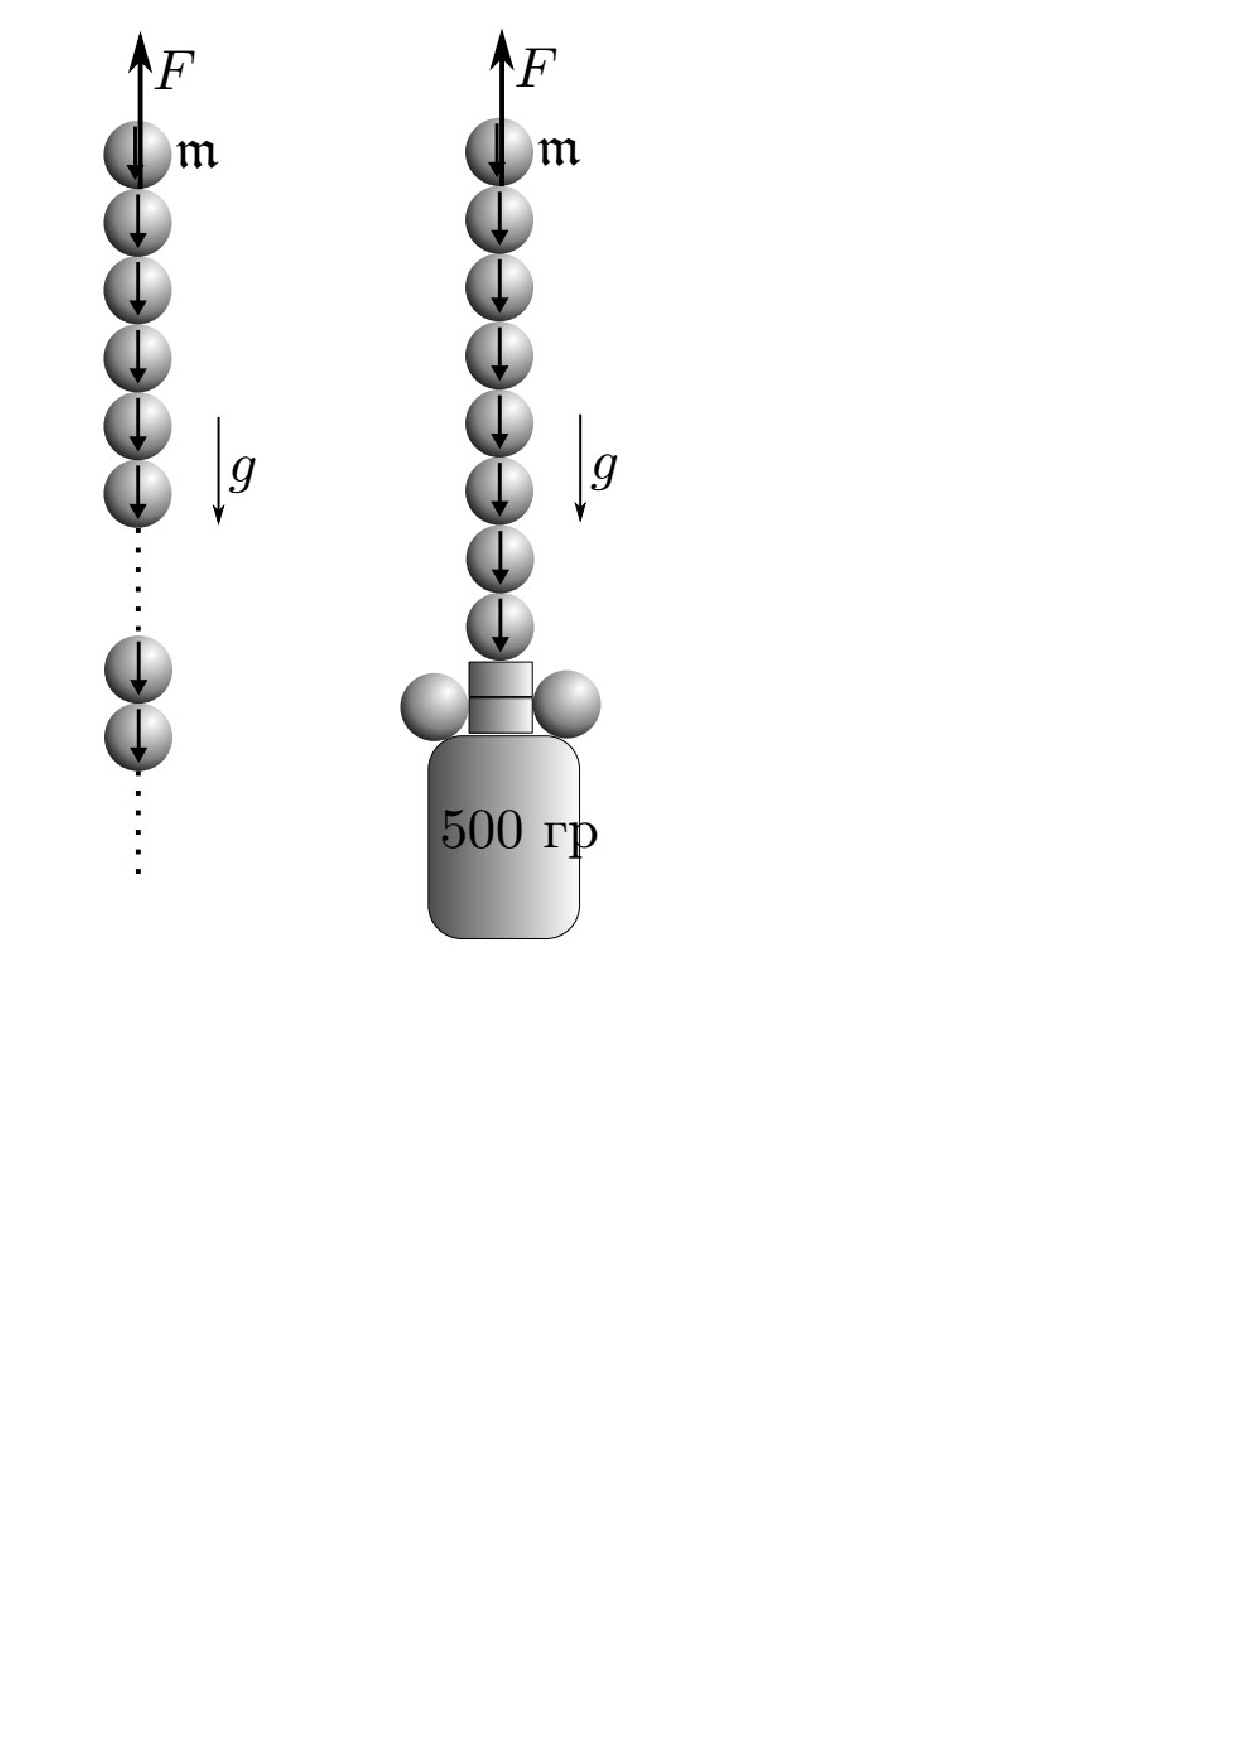
\includegraphics[width=4cm]{pics/m_chain.pdf}
	\caption{Первый способ определения магнитного момента.}
	\label{m_chain}
\end{wrapfigure}
\textbf{2-й способ} Максимальную силу сцепления можно определить по весу магнитной цепочки, кото­рую способен удержать самый верхний маг­нитный шарик. Если цепь состоит из одина­ковых магнитных шариков (см. рис. \ref{m_chain}), то при определённой длине она отрывается от верхнего шарика. При этом, учитывая, что
сила притяжения убывает как $F \propto r^{-4}$, где $r$ — расстояния между центрами шаров, для расчёта прочности цепочки достаточно учи­тывать силу взаимодействия верхнего шара с 3–4 ближайшими соседями. Сила сцепления двух одинаковых шаров радиусами $R$ c магнит­ными моментами $\m$ равна
$F_0 = \dfrac{6\m^2}{(2R)^4}=\dfrac{3\m^2}{8R^4}$. Тогда в верхней точке:
\begin{equation}
F = F_0 \left( 1 + \frac{1}{2^4} + \frac{1}{3^4} + \frac{1}{4^4} + \dots \right) \approx 1.08 F_0
\label{f0}
\end{equation}

Таким образом, найдя максимальную массу цепочки, при которой она еще не разрывается, сможем оценить величину магнитного момента шарика.

\subsection{Определение горизонтальной составляющей магнитного поля}
\begin{wrapfigure}[12]{r}{3.5cm}\vspace{-5mm}
\centering
	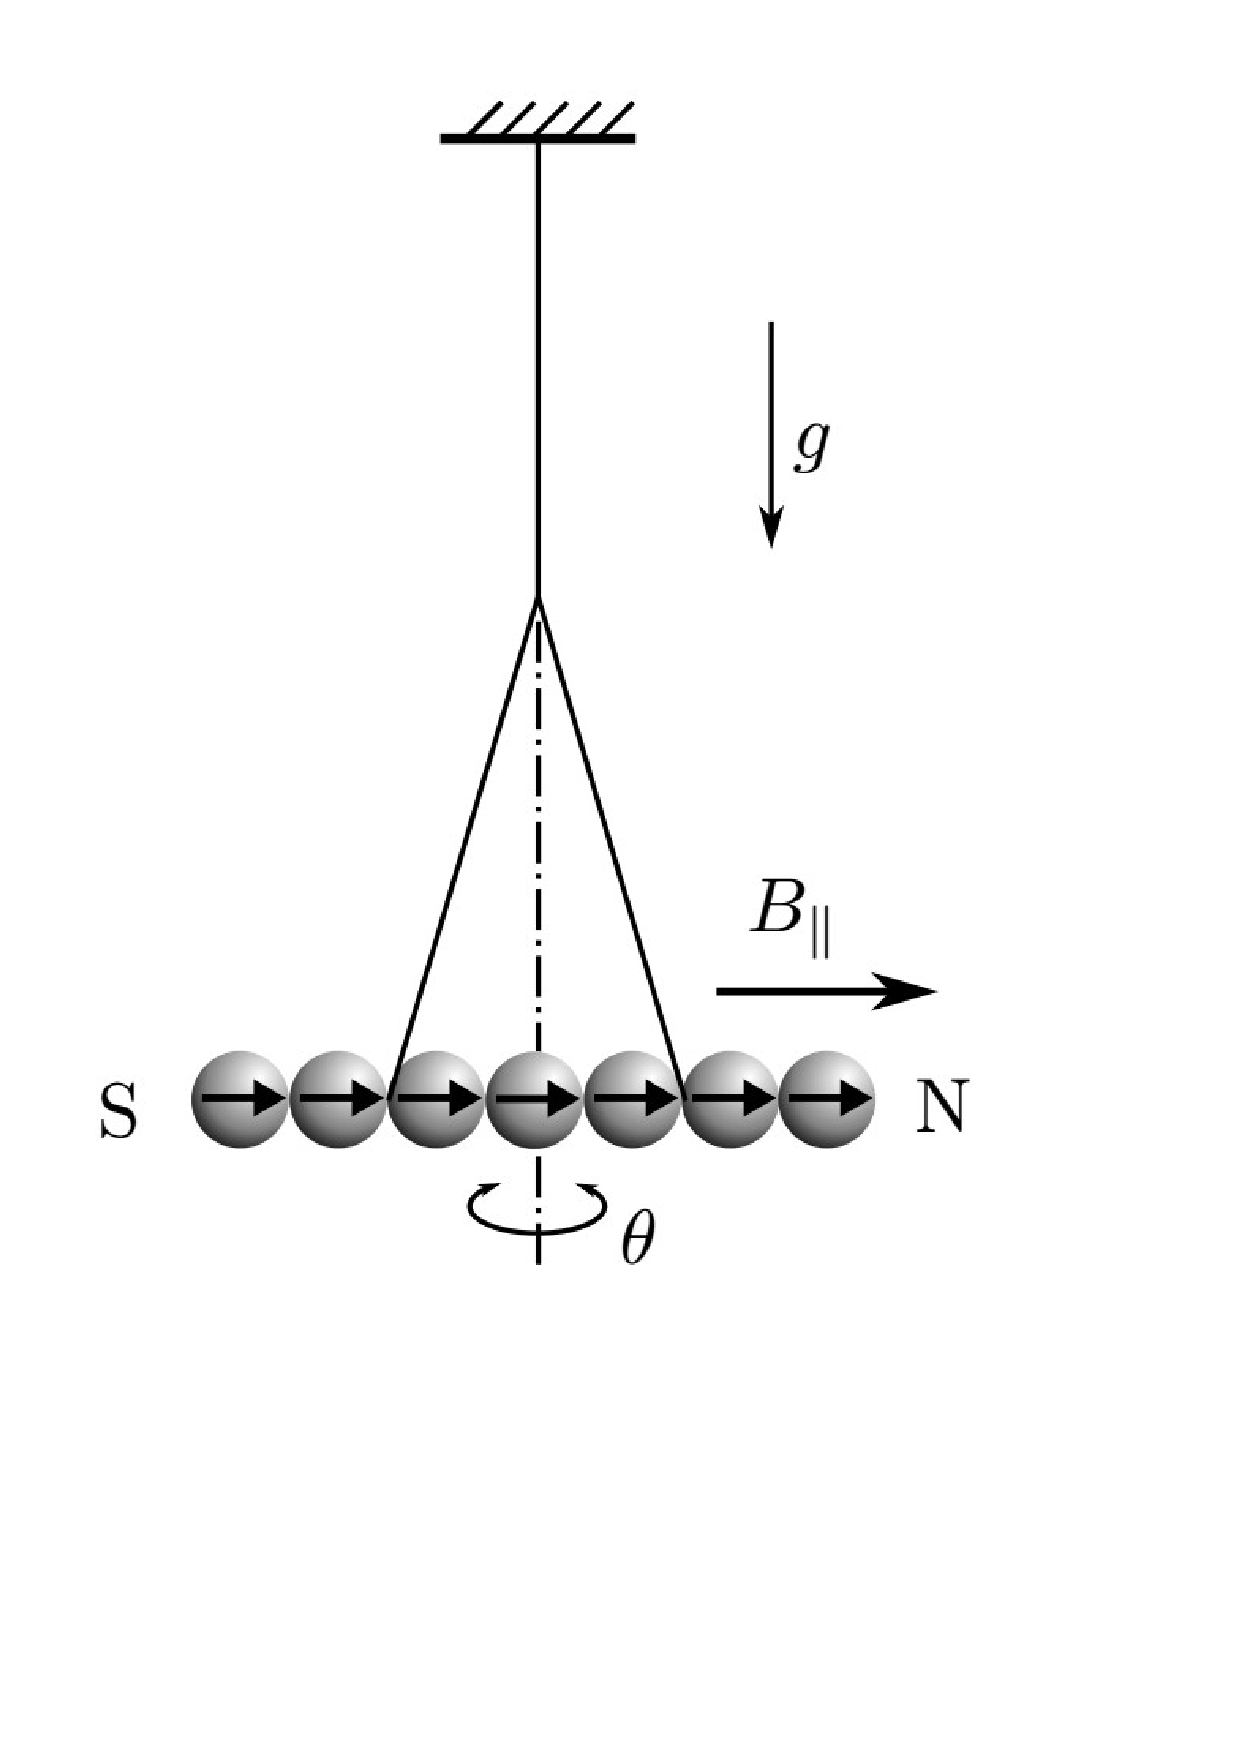
\includegraphics[width=3cm]{pics/b_par.pdf}
	\caption{Крутильный маятник}
	\label{m_chain}
\end{wrapfigure}
Магнитное поле Земли в настоящей работе измеряется по периоду
крутильных колебаний <<магнитной стрелки>> вокруг вертикальной оси.

«Магнитная стрелка» образована сцеп­ленными друг с другом $n$ намагниченными
шариками. С помощью $\mathrm{\Lambda}$-образного подвеса стрелка подвешена в горизонтальном поло­жении (см. рис. 3). Для крепления нити в работе используется штатив, изготовленный из немагнитного материала.
Тогда для $n$ шаров записав уравнение колебаний (\ref{osc}), найдём их период (\ref{period}):
\begin{equation}
J_n \ddot{\theta} + {\m}_n B_{||}\theta = 0
\label{osc}
\end{equation}
\begin{equation}
J_n \approx \frac{1}{12} m_n l_n^2 =\frac{1}{12} (m\cdot n) (2R\cdot n)^2 = \frac{1}{3} n^3 \cdot mR^2
\end{equation}
\begin{equation}
T_n = 2\pi \sqrt{\dfrac{J_n}{{\m}_n B_{||}}} = 2\pi \sqrt{\dfrac{mR^2}{3\m B_{||}}}\cdot n
\label{period}
\end{equation}

\subsection{Определение вертикальной составляющей магнитного поля}
Подвесим цепь из магнитов за центральную часть и будем уравновешивать конструкцию так, чтобы она заняла горизонтальное положение.
\begin{equation}
\mathcal{M}_n = n \m B_\perp
\label{bperpeq}
\end{equation}
\newpage
\section{Результаты измерений и~обработка данных}
Масса 30 шариков составила $30m = (25.03\pm0.01)~\mathrm{g}$, $m = (0.8343\pm0.0004)~\mathrm{g}$.
Длина цепочки из 21 шарика $(123.7 \pm 0.1)~\mathrm{mm}$, $r = (2.95 \pm 0.01)~\mathrm{mm}$.

По 1 методу измерения $\m$:
Максимальное расстояние между полюсами шариков $r_{max} - 2r = (18.6 \pm 0.1)~\mathrm{mm}$, тогда $r_{max} = (24.5 \pm 0.1)~\mathrm{mm}$. Тогда согласно (\ref{m_offset}), $\m = (70.1\pm0.6) \fcgs$, ${\varepsilon (\m) = \sqrt{\frac{1}{4}\cdot \varepsilon(m)^2 + 4\cdot \varepsilon(r_\text{max})^2} \approx 0.8 \%}$.


По 2 методу измерения $\m$:
Максимальная суммарная масса подвеса, при которой цепочка не разрывалась\footnote{Часто оказывалась, что цепочка разрывалась не посередние. В практическом смысле это значит, что шарики неидеальны и имеют некоторые отклонения в своих параметрах.}, составила $(455.2\pm 0.1)~\mathrm{g}$. Согласно (\ref{m_chain}), $\m = (91.4\pm0.4) \fcgs$, \linebreak${\varepsilon(\m) = \sqrt{4 \cdot \varepsilon(R)^2 + \frac{1}{4} \varepsilon{F}^2} \approx 0.4 \%}$.

Отметим, что оба метода неточны, так как делаются <<с рук>>, и скорее всего дают несколько заниженные результаты. Тем не менее, в попытке приблизиться к истине примем для дальнейших вычислений $\m = (81\pm 10)\fcgs$ (как среднее между двумя полученными значениями $\m$).

Проведём измерения для определения горизонтальной компоненты мангнитного поля. Измерения представлены в \textit{табл. \ref{results1}}.

\begin{table}[H]
\centering
\begin{tabular}{|l|l|l|l|l|l|l|l|l|l|l|}
\hline
$n$                      & 3     & 4     & 5     & 6     & 7     & 8     & 9     & 10    & 11    & 12    \\ \hline
$N$                      & 20    & 15    & 10    & 10    & 10    & 5     & 5     & 5     & 5     & 5     \\ \hline
$N\tau_1, \mathrm{s}$    & 18.24 & 18.61 & 16.46 & 19.08 & 23.36 & 14.04 & 15.47 & 16.67 & 17.58 & 19.79 \\ \hline
$N\tau_2, \mathrm{s}$    & 18.34 & 18.94 & 16.51 & 19.22 & 23.25 & 14.01 & 15.09 & 17.08 & 17.24 & 19.43 \\ \hline
$N\tau_3, \mathrm{s}$    & 18.40 & 19.10 & 16.32 & 18.94 & 23.03 & 14.12 & 15.11 & 16.44 & 17.35 & 19.96 \\ \hline
$\tau, \mathrm{s}$ & 0.916 & 1.259 & 1.643 & 1.908 & 2.321 & 2.811 & 3.045 & 3.346 & 3.478 & 3.945 \\ \hline
$\sigma({\tau}), \mathrm{s}$         & 0.020 & 0.020 & 0.020 & 0.020 & 0.020 & 0.020 & 0.020 & 0.020 & 0.020 & 0.020 \\ \hline
\end{tabular}
\caption{Результаты измерения периодов колебаний}
\label{results1}
\end{table}
По полученным данным построим график (\ref{plot_tn_n}):
\begin{figure}[H]
\centering
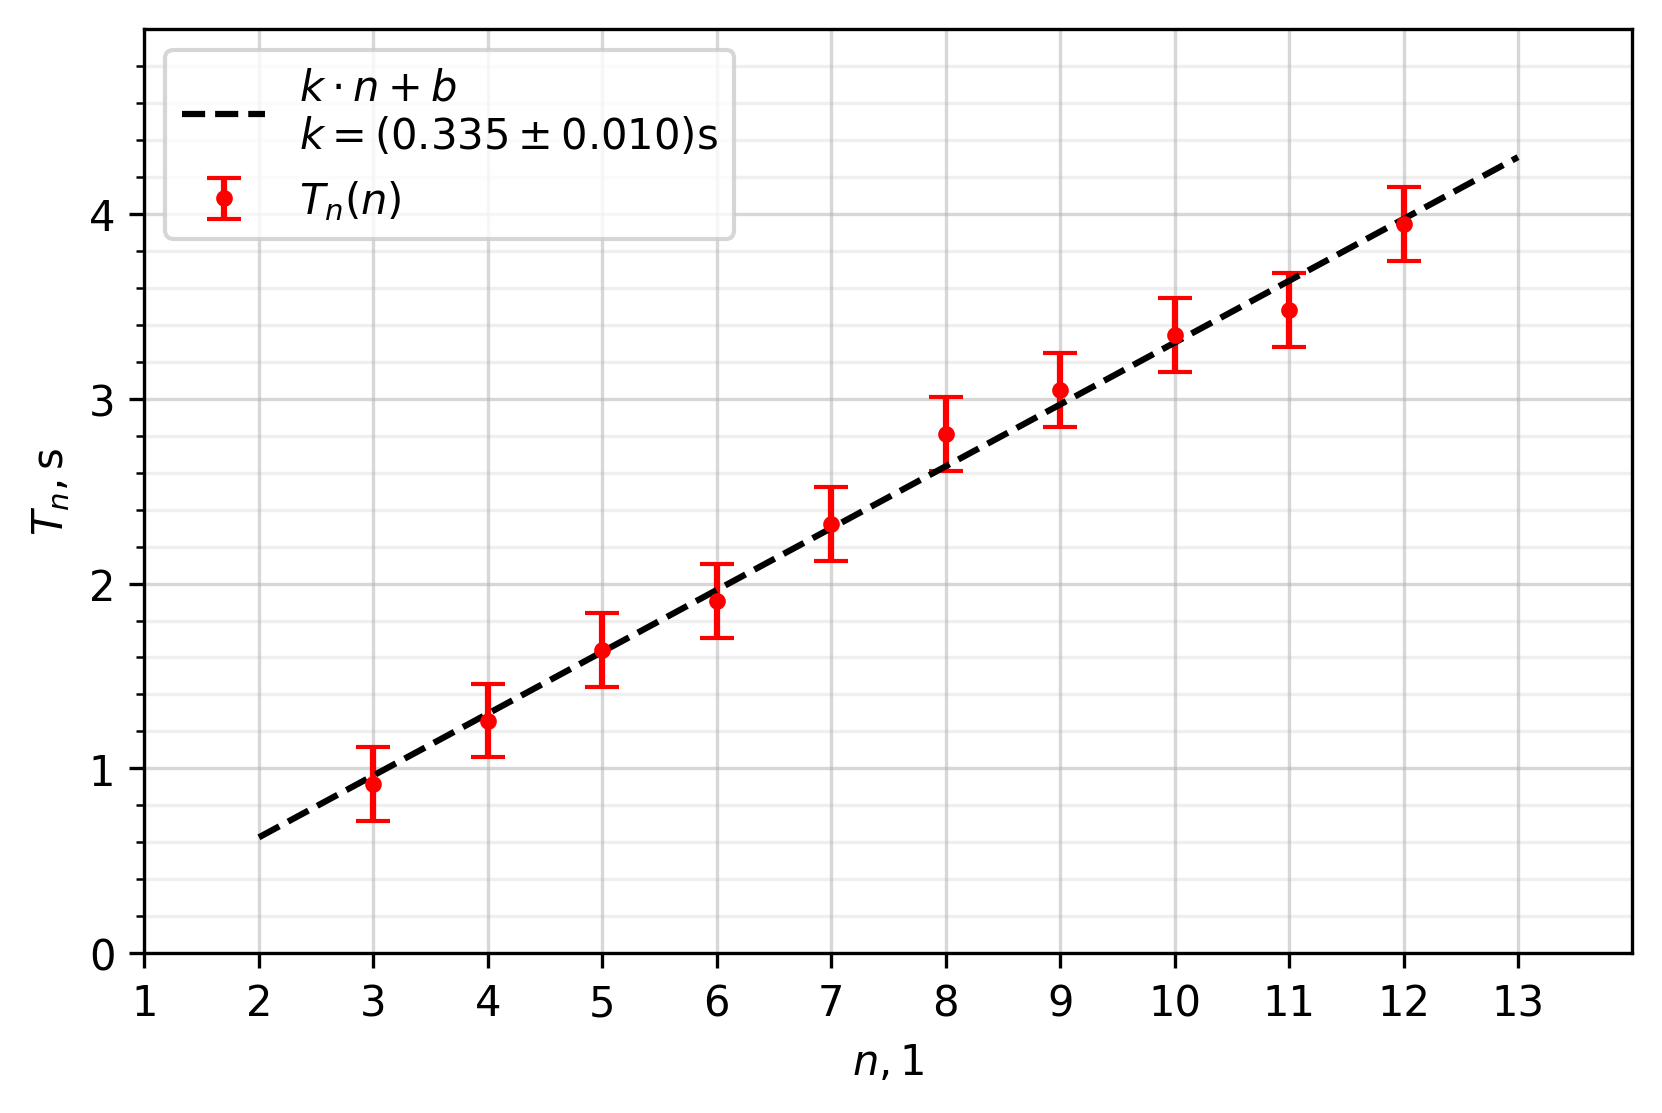
\includegraphics[width=0.8\linewidth]{pics/plot_tn_n.png}
\caption{График зависимости периода колебаний в поле от количества шариков}
\label{plot_tn_n}
\end{figure}
Согласно (\ref{period}), получаем:
\begin{equation}
B_{||} = \dfrac{4\pi^2 mR^2}{3\m k^2} = (105\pm 13)~\mathrm{mG} = (1.05\pm 0.13)\cdot 10^{-5}~\mathrm{T}
\end{equation}

Теперь перейдём к вычислению наклонения магнитного поля.
Выберем 4 куска проволоки и найдём их параметры. Диаметр проволоки составил $d=0.26~\mathrm{mm}$, плотность меди $\rho = 8.96~\mathrm{g/cm^3}$.
\begin{table}[H]
\centering
\begin{tabular}{|l|l|l|l|l|}
\hline
Образец          & 1    & 2    & 3    & 4    \\ \hline
$L, \mathrm{cm}$ & 16.9 & 18.0 & 6.5  & 9.0  \\ \hline
$m, \mathrm{mg}$ & 80.4 & 85.6 & 30.9 & 42.8 \\ \hline
\end{tabular}
\caption{Параметры проволочек}
\end{table}

Тогда будем находить такие конфигурации подвеса проволок, при которых подвес будет ближе всего к горизонтальному положению. Знак <<+>> будет означать подвешивание против изначального крена, <<->> -- соответственно, в направлении крена.

\begin{table}[H]
\begin{tabular}{|l|l|l|l|l|l|}
\hline
$n, 1$                                 & 12   & 10 & 8      & 6      & 4      \\ \hline
$l_{подвес}, R$                        & 5    & 4  & 3      & 2      & 1      \\ \hline
Конфигурация                           & +1+4 & +1 & +1+2-3 & +1+2-4 & +1+2-4 \\ \hline
$\mathcal{M}, \text{dyn}\cdot\text{cm}$ & 178  & 93 & 117    & 71     & 36     \\ \hline
\end{tabular}
\end{table}

\begin{figure}[H]
\centering
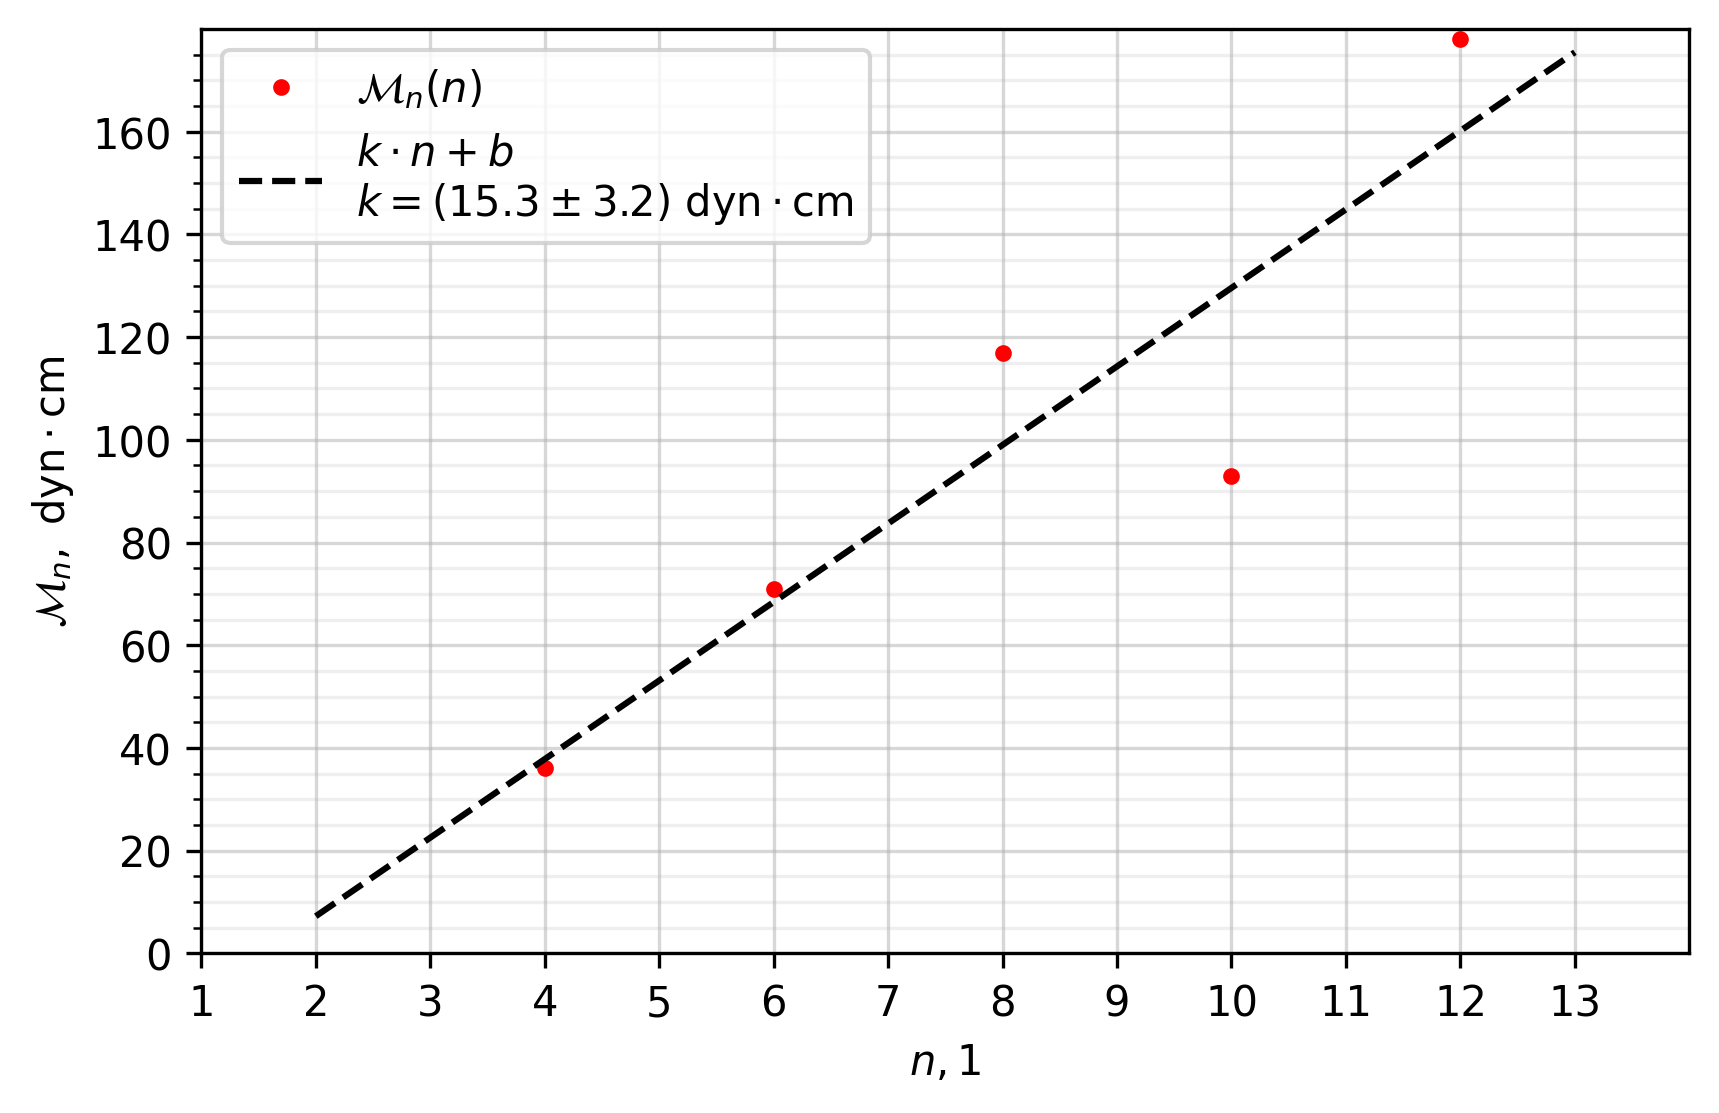
\includegraphics[width=0.8\linewidth]{pics/plot_mn_n.png}
\caption{График зависимости уравновешивающего момента от количества шариков}
\label{plot_mn_n}
\end{figure}
Погрешности на графике не приводятся, так как они несущественны по сравнению со статистическим разбросом. 
Согласно (\ref{bperpeq}), найдем $B_\perp = (190\pm50)~\text{mG}$.

\newpage
\section{Обсуждение результатов}
Обратившись к \cite{wmc}, найдём табличные значения магнитного поля в Москве и сравним с полученными результатами:
\begin{table}[H]
\begin{tabular}{|l|l|l|}
\hline
                 & $B_{||},~\mathrm{\mu T}$ & $B_{\perp},~\mathrm{\mu T}$ \\ \hline
Табличные данные & 16.6 & 50.3   \\ \hline
Эксперимент      &  $(10.5\pm 1.3)$    &   $(19\pm 5)$   \\ \hline
\end{tabular}
\end{table}

Результат эксперимента можно описать как удовлетворительный -- несмотря на попадание величин в порядок, расхождение с табличными данными кратное.  Напомним, что заметное расхождение началось еще при различных методах измерения $\m$. Как задача-оценка, в целом, эксперимент удался.

\section{Выводы}
Были проведены измерения магнитного момента идентичных магнитов и с помощью них измерена индукция магнитного поля Земли. Результат получился оценочный, но попадающий в порядок величины.

\begin{thebibliography}{}
     \bibitem{wmc}  \textbf{WMC} -- http://www.geomag.bgs.ac.uk/data\_service/models\_compass/wmm\_calc.html
\end{thebibliography}
\end{document}
